
\section{Knowledge and reasoning distillation} \label{sec:distillation}

%% \begin{figure}
%%   \centering
%%   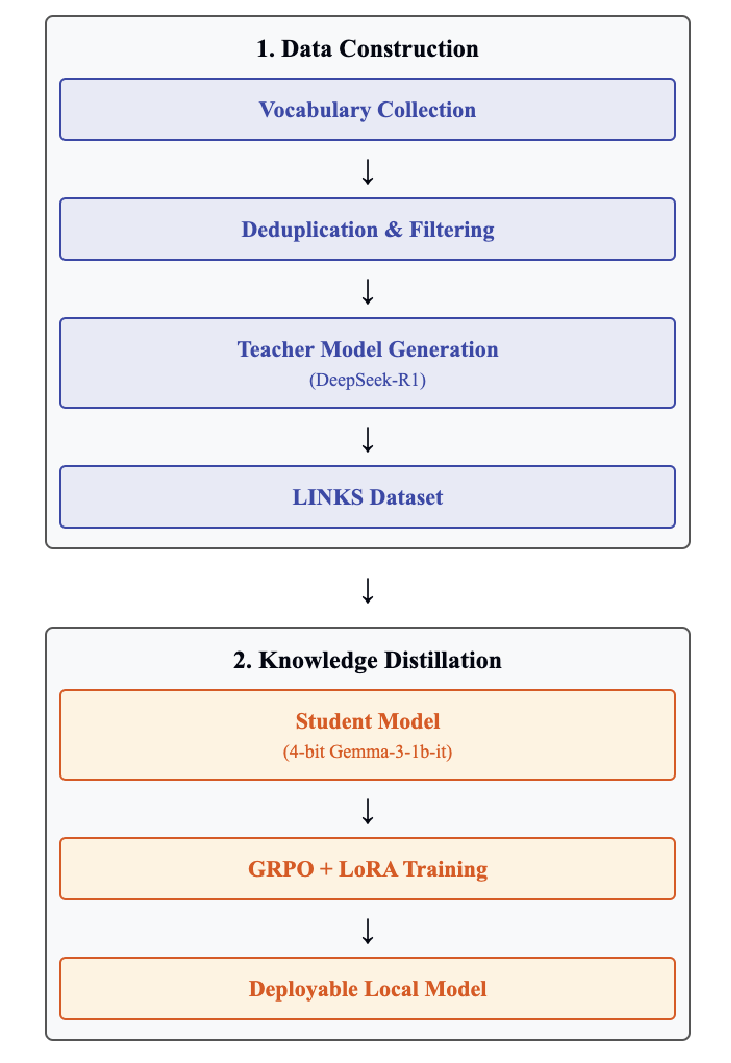
\includegraphics[width=\linewidth]{figures/pipeline.pdf}
%%   \caption{\links pipeline. The pipeline consists of two main components: (1) CoT data generation and (2) model distillation. In the first step, we generate a dataset of mnemonics with reasoning traces using a large language model (LLM) as a teacher. In the second step, we distill the reasoning capabilities of the teacher model into a smaller student model using GRPO \Cref{app:grpo}. The final model can be deployed locally for vocabulary learning tasks.}
%%   \label{fig:distillation}
%% \end{figure}

We present \links, a pipeline that distills linguistic knowledge and reasoning through a teacher-student framework. This approach generates linguistically grounded mnemonics with reasoning traces and exemplifying sentences for vocabulary learning.

\subsection{Data construction} \label{sec:data-gen}
To generate high-quality linguistically grounded mnemonics, we first created a comprehensive training dataset. Following best practices in synthetic data generation with LLMs \citetext{\citealp{longLLMsDrivenSyntheticData2024b}, \citealp{openthoughtsteamOpenThoughts2025}}, we designed a data construction pipeline with several key components.

\paragraph{Vocabulary collection} We collected 5,000 distinct vocabulary words from four complementary sources: English as a foreign language tests (TOEFL iBT, IELTS Academic), standardized tests (SAT, GRE), CEFR levels C1 and C2 word lists, and the Oxford Dictionary of Philosophy. We selected these sources to ensure coverage of academic and abstract vocabulary that would benefit from mnemonic devices. After deduplication and fuzzy-matching decontamination, we refined our dataset to 2,000 distinct vocabulary words for post-training.

\paragraph{Prompt design} Based on the findings from \cref{sec:icl-performance}, we crafted system and user prompts that encouraged linguistically grounded reasoning. Our system prompt instructed the model to analyze potential linguistic features before generating a mnemonic. We used structured output format with designated sections for reasoning, mnemonic, and example, allowing for clearer evaluation and potential future extraction of specific components.

\paragraph{Teacher model selection} We selected \teachermodel (670B parameters) \citep{DeepSeek-AIDEEPSEEKR12025} for its advanced reasoning capabilities and extensive knowledge as the teacher model.

\paragraph{Dataset generation} Using the designed prompts and vocabulary list, we generated the \links, a dataset of approximately 2,000 entries, each containing: (1) a detailed reasoning trace exploring multiple linguistic features of the target vocabulary, (2) a concise mnemonic device leveraging the most salient linguistic connection, and, (3) an exemplifying sentence demonstrating proper usage.

\paragraph{Quality control} To ensure the quality of the generated mnemonics, we implemented a multi-step validation process. We first filtered out any entries that did not meet our structured output format or contained incomplete reasoning traces. We then performed a manual review of a random sample of 200 entries to assess the linguistic grounding and coherence of the mnemonics. This review process involved checking for clear connections between the vocabulary and the mnemonic, as well as ensuring that the example sentence accurately reflected the vocabulary's meaning.

\subsection{Training and inference} \label{sec:training-inference}
After generating the synthetic dataset, we implemented a distillation process to transfer this linguistic reasoning capability to a smaller, easier-to-deploy model.

\paragraph{Student model selection} We selected \studentmodel as our student model due to its balance of performance, size, and deployment flexibility. This instruction-tuned variant of Google's Gemma-3 (1 billion parameters) \citep{GemmaTeamGEMMA2025} offers several advantages: (1) demonstrated instruction-following abilities, (2) multilingual capabilities for potential cross-lingual applications, and (3) compact size enabling deployment on consumer hardware including Apple Silicon.

\paragraph{Group Relative Policy Optimization (GRPO)} We employed GRPO \citep{DeepSeek-AIDEEPSEEKR12025} to distill the reasoning capabilities of the teacher model into the student model. The GRPO process consists of three main steps: (1) generating multiple candidate outputs for each input, (2) scoring these outputs using a reward model(s), and (3) updating the student model's policy based on the scores. GRPO technical details are included in \Cref{app:grpo}  and our used configuration is provided in \Cref{app:grpo}.

We defined three reward functions that encode basic characteristics of effective mnemonics:
(1) adherence to the structured format with reasoning, mnemonic, and example,
(2) explicit incorporation of linguistic features in \Cref{tab:linguistic-features}, and
(3) usage of the target vocabulary in the mnemonic,  penalizing bad mnemonics such as acronyms.
These reward functions operate directly on model outputs, assigning scalar scores based on how well the generation satisfies each criterion. The scores are then combined using weighted summation, with higher weights assigned to criteria 1 and 2. We generated two candidate outputs per training example to enable reinforcement from comparisons. Training was performed on a single NVIDIA H100 GPU approximately 4 hours.

\paragraph{Low-Rank Adaptation (LoRA)} We trained \studentmodel using GRPO wrapped in LoRA layers (\Cref{app:peft}) to reduce the number of trainable parameters and rank-stabilized LoRA that maintains stability for adapters with higher ranks. Full LoRA configuration is provided in \Cref{app:lora-config}.

\paragraph{Model quantization and serving} To enable efficient deployment on consumer hardware, we quantized the final model using 4-bit quantization with the NormalFloat (NF4) data type \citep{dettmersQLoRAEfficientFinetuning2023}. This significantly reduced the model size while maintaining performance quality. The quantized model can be served with a local application such as OpenWebUI (interface) and Ollama (command-line), making it accessible for language learners without requiring continuous internet connectivity or sharing potentially sensitive language learning data with third-party services.
